\documentclass[16pt]{beamer}
\usepackage[utf8]{inputenc}
\usepackage[T1]{fontenc}
\usepackage{graphicx}
\usepackage[polish]{babel}
\usepackage{url}
\usepackage{fancyvrb}
\usepackage{color}

\makeatletter
\def\PY@reset{\let\PY@it=\relax \let\PY@bf=\relax%
    \let\PY@ul=\relax \let\PY@tc=\relax%
    \let\PY@bc=\relax \let\PY@ff=\relax}
\def\PY@tok#1{\csname PY@tok@#1\endcsname}
\def\PY@toks#1+{\ifx\relax#1\empty\else%
    \PY@tok{#1}\expandafter\PY@toks\fi}
\def\PY@do#1{\PY@bc{\PY@tc{\PY@ul{%
    \PY@it{\PY@bf{\PY@ff{#1}}}}}}}
\def\PY#1#2{\PY@reset\PY@toks#1+\relax+\PY@do{#2}}

\def\PY@tok@gd{\def\PY@tc##1{\textcolor[rgb]{0.63,0.00,0.00}{##1}}}
\def\PY@tok@gu{\let\PY@bf=\textbf\def\PY@tc##1{\textcolor[rgb]{0.50,0.00,0.50}{##1}}}
\def\PY@tok@gt{\def\PY@tc##1{\textcolor[rgb]{0.00,0.25,0.82}{##1}}}
\def\PY@tok@gs{\let\PY@bf=\textbf}
\def\PY@tok@gr{\def\PY@tc##1{\textcolor[rgb]{1.00,0.00,0.00}{##1}}}
\def\PY@tok@cm{\let\PY@it=\textit\def\PY@tc##1{\textcolor[rgb]{0.25,0.50,0.50}{##1}}}
\def\PY@tok@vg{\def\PY@tc##1{\textcolor[rgb]{0.10,0.09,0.49}{##1}}}
\def\PY@tok@m{\def\PY@tc##1{\textcolor[rgb]{0.40,0.40,0.40}{##1}}}
\def\PY@tok@mh{\def\PY@tc##1{\textcolor[rgb]{0.40,0.40,0.40}{##1}}}
\def\PY@tok@go{\def\PY@tc##1{\textcolor[rgb]{0.50,0.50,0.50}{##1}}}
\def\PY@tok@ge{\let\PY@it=\textit}
\def\PY@tok@vc{\def\PY@tc##1{\textcolor[rgb]{0.10,0.09,0.49}{##1}}}
\def\PY@tok@il{\def\PY@tc##1{\textcolor[rgb]{0.40,0.40,0.40}{##1}}}
\def\PY@tok@cs{\let\PY@it=\textit\def\PY@tc##1{\textcolor[rgb]{0.25,0.50,0.50}{##1}}}
\def\PY@tok@cp{\def\PY@tc##1{\textcolor[rgb]{0.74,0.48,0.00}{##1}}}
\def\PY@tok@gi{\def\PY@tc##1{\textcolor[rgb]{0.00,0.63,0.00}{##1}}}
\def\PY@tok@gh{\let\PY@bf=\textbf\def\PY@tc##1{\textcolor[rgb]{0.00,0.00,0.50}{##1}}}
\def\PY@tok@ni{\let\PY@bf=\textbf\def\PY@tc##1{\textcolor[rgb]{0.60,0.60,0.60}{##1}}}
\def\PY@tok@nl{\def\PY@tc##1{\textcolor[rgb]{0.63,0.63,0.00}{##1}}}
\def\PY@tok@nn{\let\PY@bf=\textbf\def\PY@tc##1{\textcolor[rgb]{0.00,0.00,1.00}{##1}}}
\def\PY@tok@no{\def\PY@tc##1{\textcolor[rgb]{0.53,0.00,0.00}{##1}}}
\def\PY@tok@na{\def\PY@tc##1{\textcolor[rgb]{0.49,0.56,0.16}{##1}}}
\def\PY@tok@nb{\def\PY@tc##1{\textcolor[rgb]{0.00,0.50,0.00}{##1}}}
\def\PY@tok@nc{\let\PY@bf=\textbf\def\PY@tc##1{\textcolor[rgb]{0.00,0.00,1.00}{##1}}}
\def\PY@tok@nd{\def\PY@tc##1{\textcolor[rgb]{0.67,0.13,1.00}{##1}}}
\def\PY@tok@ne{\let\PY@bf=\textbf\def\PY@tc##1{\textcolor[rgb]{0.82,0.25,0.23}{##1}}}
\def\PY@tok@nf{\def\PY@tc##1{\textcolor[rgb]{0.00,0.00,1.00}{##1}}}
\def\PY@tok@si{\let\PY@bf=\textbf\def\PY@tc##1{\textcolor[rgb]{0.73,0.40,0.53}{##1}}}
\def\PY@tok@s2{\def\PY@tc##1{\textcolor[rgb]{0.73,0.13,0.13}{##1}}}
\def\PY@tok@vi{\def\PY@tc##1{\textcolor[rgb]{0.10,0.09,0.49}{##1}}}
\def\PY@tok@nt{\let\PY@bf=\textbf\def\PY@tc##1{\textcolor[rgb]{0.00,0.50,0.00}{##1}}}
\def\PY@tok@nv{\def\PY@tc##1{\textcolor[rgb]{0.10,0.09,0.49}{##1}}}
\def\PY@tok@s1{\def\PY@tc##1{\textcolor[rgb]{0.73,0.13,0.13}{##1}}}
\def\PY@tok@sh{\def\PY@tc##1{\textcolor[rgb]{0.73,0.13,0.13}{##1}}}
\def\PY@tok@sc{\def\PY@tc##1{\textcolor[rgb]{0.73,0.13,0.13}{##1}}}
\def\PY@tok@sx{\def\PY@tc##1{\textcolor[rgb]{0.00,0.50,0.00}{##1}}}
\def\PY@tok@bp{\def\PY@tc##1{\textcolor[rgb]{0.00,0.50,0.00}{##1}}}
\def\PY@tok@c1{\let\PY@it=\textit\def\PY@tc##1{\textcolor[rgb]{0.25,0.50,0.50}{##1}}}
\def\PY@tok@kc{\let\PY@bf=\textbf\def\PY@tc##1{\textcolor[rgb]{0.00,0.50,0.00}{##1}}}
\def\PY@tok@c{\let\PY@it=\textit\def\PY@tc##1{\textcolor[rgb]{0.25,0.50,0.50}{##1}}}
\def\PY@tok@mf{\def\PY@tc##1{\textcolor[rgb]{0.40,0.40,0.40}{##1}}}
\def\PY@tok@err{\def\PY@bc##1{\fcolorbox[rgb]{1.00,0.00,0.00}{1,1,1}{##1}}}
\def\PY@tok@kd{\let\PY@bf=\textbf\def\PY@tc##1{\textcolor[rgb]{0.00,0.50,0.00}{##1}}}
\def\PY@tok@ss{\def\PY@tc##1{\textcolor[rgb]{0.10,0.09,0.49}{##1}}}
\def\PY@tok@sr{\def\PY@tc##1{\textcolor[rgb]{0.73,0.40,0.53}{##1}}}
\def\PY@tok@mo{\def\PY@tc##1{\textcolor[rgb]{0.40,0.40,0.40}{##1}}}
\def\PY@tok@kn{\let\PY@bf=\textbf\def\PY@tc##1{\textcolor[rgb]{0.00,0.50,0.00}{##1}}}
\def\PY@tok@mi{\def\PY@tc##1{\textcolor[rgb]{0.40,0.40,0.40}{##1}}}
\def\PY@tok@gp{\let\PY@bf=\textbf\def\PY@tc##1{\textcolor[rgb]{0.00,0.00,0.50}{##1}}}
\def\PY@tok@o{\def\PY@tc##1{\textcolor[rgb]{0.40,0.40,0.40}{##1}}}
\def\PY@tok@kr{\let\PY@bf=\textbf\def\PY@tc##1{\textcolor[rgb]{0.00,0.50,0.00}{##1}}}
\def\PY@tok@s{\def\PY@tc##1{\textcolor[rgb]{0.73,0.13,0.13}{##1}}}
\def\PY@tok@kp{\def\PY@tc##1{\textcolor[rgb]{0.00,0.50,0.00}{##1}}}
\def\PY@tok@w{\def\PY@tc##1{\textcolor[rgb]{0.73,0.73,0.73}{##1}}}
\def\PY@tok@kt{\def\PY@tc##1{\textcolor[rgb]{0.69,0.00,0.25}{##1}}}
\def\PY@tok@ow{\let\PY@bf=\textbf\def\PY@tc##1{\textcolor[rgb]{0.67,0.13,1.00}{##1}}}
\def\PY@tok@sb{\def\PY@tc##1{\textcolor[rgb]{0.73,0.13,0.13}{##1}}}
\def\PY@tok@k{\let\PY@bf=\textbf\def\PY@tc##1{\textcolor[rgb]{0.00,0.50,0.00}{##1}}}
\def\PY@tok@se{\let\PY@bf=\textbf\def\PY@tc##1{\textcolor[rgb]{0.73,0.40,0.13}{##1}}}
\def\PY@tok@sd{\let\PY@it=\textit\def\PY@tc##1{\textcolor[rgb]{0.73,0.13,0.13}{##1}}}

\def\PYZbs{\char`\\}
\def\PYZus{\char`\_}
\def\PYZob{\char`\{}
\def\PYZcb{\char`\}}
\def\PYZca{\char`\^}
% for compatibility with earlier versions
\def\PYZat{@}
\def\PYZlb{[}
\def\PYZrb{]}
\makeatother


\usetheme{Pittsburgh}
\usenavigationsymbolstemplate{} % turn off navigation icons
\setbeamercovered{transparent}

\author{Silesian Ruby Users Group\\\footnotesize{Jakub Kuźma}}
\title{Lisp - Introduction}

\begin{document}

\frame{\titlepage}

\begin{frame}
  \frametitle{WTF?}
  \begin{center}
    Lisp?!?
  \end{center}
\end{frame}

\begin{frame}
  \frametitle{Lisp Dialects}
  \begin{itemize}
  \item Common Lisp (gcl)
  \item Scheme (guile)
  \item Clojure (JVM)
  \item AutoLISP (AutoCAD)
  \item Emacs Lisp (Emacs)
  \end{itemize}
\end{frame}

\begin{frame}
  \frametitle{John McCarthy\\September 4, 1927 -- October 24, 2011}
  \begin{figure}
    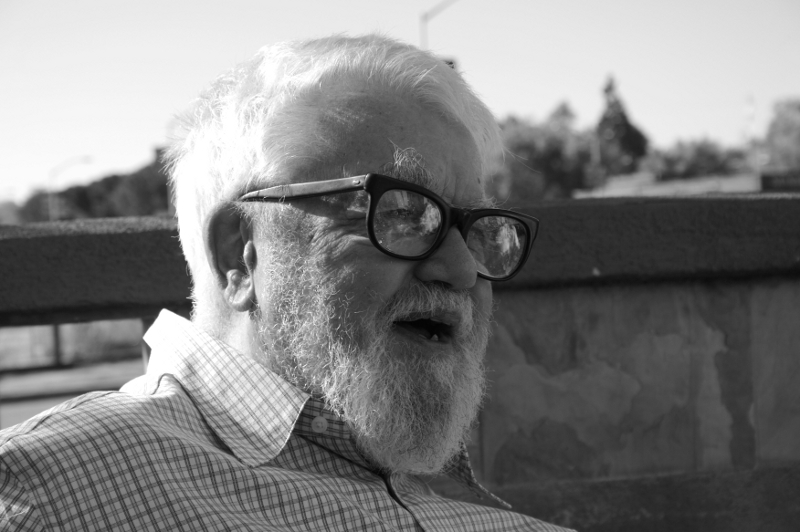
\includegraphics[width=0.8\linewidth]{mccarthy.jpg}
  \end{figure}
\end{frame}

\begin{frame}
  \frametitle{Atoms}
  \begin{block}{}
    Atoms are strings of letters and digits and other characters not
    otherwise used in Lisp.
  \end{block}
  \begin{itemize}
  \item 0, 42, 3.14
  \item ``hello, world!''
  \item foo, car, +
  \item nil, t
  \end{itemize}
\end{frame}

\begin{frame}
  \frametitle{Lists}
  \begin{block}{}
    A list consist of a left parenthesis followed by zero or more
    atoms or lists separated by spaces and ending with a right
    parenthesis.
  \end{block}
  \begin{itemize}
  \item ()
  \item (foo)
  \item (1 + 2)
  \item (foo (bar (baz)))
  \end{itemize}
\end{frame}

\begin{frame}
  \frametitle{Symbolic Expressions}
  \begin{block}{}
    Not all s-expressions are valid Lisp programs.
  \end{block}
\end{frame}

\begin{frame}
  \frametitle{Primitives}
  \begin{itemize}
  \item (quote $e$)
  \item (car $e$)
  \item (cdr $e$)
  \item (cons $e_1$ $e_2$)
  \item (equal $e_1$ $e_2$)
  \item (atom $e$)
  \item (cond ($p_1$ $e_1$) ... ($p_n$ $e_n$))
  \item An atom $v$, regarded as a variable, may have a value.
  \item ((lambda ($v_1$ ... $v_n$) $e$) $e_1$ ... $e_n$)
  \item ((label $f$ (lambda ($v_1$ ... $v_n$) $e$)) $e_1$ ... $e_n$)
  \end{itemize}
\end{frame}

\begin{frame}
  \frametitle{Cons cell}
  \begin{figure}
    \includegraphics[width=0.6\linewidth]{cons.pdf}
  \end{figure}
\end{frame}

\begin{frame}
  \frametitle{List, first example}
  \begin{figure}
    \includegraphics[width=0.6\linewidth]{list-1.pdf}
  \end{figure}
  \begin{itemize}
  \item (cons 1 nil)
  \item (1 . nil)
  \item (1)
  \end{itemize}
\end{frame}

\begin{frame}
  \frametitle{List, second example}
  \begin{figure}
    \includegraphics[width=0.6\linewidth]{list-2.pdf}
  \end{figure}
  \begin{itemize}
  \item (cons 1 (cons 2 (cons 3 nil)))
  \item (1 . (2 . (3 . nil)))
  \item (1 2 3)
  \end{itemize}
\end{frame}

\begin{frame}
  \frametitle{List, third example}
  \begin{figure}
    \includegraphics[width=0.6\linewidth]{list-3.pdf}
  \end{figure}
  \begin{itemize}
  \item (cons (cons 1 2) (cons 3 4))
  \item ((1 . 2) . (3 . 4))
  \item ((1 . 2) 3 . 4)
  \end{itemize}
\end{frame}

\begin{frame}
  \frametitle{Calling functions}
  \begin{block}{}
    The most common way of invoking a function in Lisp is by
    evaluating a list. Others are: funcall, apply, etc.
  \end{block}
  \begin{itemize}
  \item (+ 2 2)
  \item (* (+ 1 3) 5)
  \item (concat ``a'' ``b'')
  \end{itemize}
\end{frame}

\begin{frame}
  \frametitle{Defining functions}
  \begin{itemize}
  \item anonymous: (lambda (a b) (+ a b))
  \item named: (defun double (x) (* 2 x))
  \end{itemize}
\end{frame}

\begin{frame}
  \frametitle{Defining variables}
  \begin{itemize}
  \item (set 'x 1)
  \item (setq x 1)
  \end{itemize}
\end{frame}

\begin{frame}
  \frametitle{Bindings}
  \begin{block}{}
  A ``binding'' is a relationship of
  correspondence between a name and a memory location.
  \end{block}
  \begin{itemize}
  \item ((lambda (a b) (...)) 1 3)
  \item (let (x y z) (...))
  \item (let ((a 1) (b 2)) (...))
  \end{itemize}
\end{frame}

\begin{frame}
  \frametitle{Conditions}
  \begin{itemize}
  \item (cond ((= x 0) 1) (t x))
  \item (if (= x 0) 1 x)
  \item (unless (> x 0) (print x))
  \end{itemize}
\end{frame}

\begin{frame}
  \frametitle{Collections}
  \begin{itemize}
  \item lists: (1 2 3 4 5)
  \item arrays: [1 2 3 4]
  \item hashes: (make-hash-table)
  \end{itemize}
\end{frame}

\begin{frame}
  \frametitle{Macros}
  \begin{block}{}
  Macros are programs that generate programs.
  \end{block}
  \begin{itemize}
  \item (loop for i from 1 to 10 do (print i) finally return 1)
  \end{itemize}
\end{frame}

\begin{frame}
  \frametitle{Books}
  \begin{itemize}
  \item Land of Lisp -- Conrad Barski
  \item Practical Common Lisp -- Peter Seibel
  \end{itemize}
\end{frame}

\begin{frame}
  \frametitle{Questions?}
  \begin{center}
  CAN HAS QUESTIONS?
  \end{center}
\end{frame}

\end{document}

